

\chapter{Results}

\label{Chapter6}
This chapter contains the results from all the implementations provided with some assessment of them along with any interesting findings in the process. There will also be comparisons where appropriate as well as trying to figure out why exactly the results are the way they are. 


It's important that before looking at the results there is an acknowledged method of deciding how \textit{good} the results are. 
The first obvious unit of measurement would be accuracy. To see how accurately the designed model predicts the classes of the data. This is the primary value needed to be as high as possible to avoid mistakes. The secondary feature would be time taken to run. This isn't as much of an issue in this experimental setting, however if this sort of system were to be attempted to integrate into other live systems, it is definitely a variable to keep in mind. 
\\
\\
There are a handful of tunable parameters for all the systems designed. To illustrate exactly which systems contain which parameters refer to the following table:


\begin{center}
\begin{tabular}{|c | m{7cm} | c |}
\hline
Parameter & Description & Used in \\
\hline
Number of features & The maximum number of features to be considered when building a tree  & Random forest \& Sklearn \\
\hline
Maximum depth & The maximum depth a tree can have along any path & forest \& Sklearn \\
\hline
Minimum size & The minimum number of nodes required to be present on both sides after a split for it to occur & Random forest \\
\hline
Sample size & The ratio of the subsample that we pick for the bagging process of building a tree & Random forest \\
\hline
Number of trees & The number of trees built in the forest & forest \& Sklearn \\
\hline
Number of folds & The number of folds used in cross validation & Random forest \\
\hline
Epochs & The number of learning cycles done for training & Neural network \\
\hline
Batch size & The number of training examples used in one iteration & Neural network \\
\hline

\end{tabular}
\textit{Table 6.1: Table of tunable parameters}
\end{center}

\section{Random Forest without Sklearn}
The following results are a varying range of accuracies based on some of the parameters being changed around. Most of the parameters have been altered at times to see what difference they make and seeing what combination of parameters give the best results.

Results for random forest implementation without sklearn:
\begin{center}
\begin{tabular}{|c | c | c | c | c | c | c |}
\hline
Trees & Maximum depth & Minimum size & Features & Folds & Sample size & Accuracy \\
\hline
2 & 5 & 1 & $\sqrt{features}$ & 2 & 1.0 & 90.7\% \\
\hline
5 & 5 & 1 & $\sqrt{features}$ & 2 & 1.0 & 92.0\% \\
\hline
10 & 5 & 1 & $\sqrt{features}$ & 2 & 1.0 & 92.4\% \\
\hline
2 & 10 & 5 & $\sqrt{features}$ & 2 & 1.0 & 92.8\% \\
\hline
5 & 10 & 5 & $\sqrt{features}$ & 2 & 1.0 & 96.0\% \\
\hline
10 & 10 & 5 & $\sqrt{features}$ & 2 & 1.0 & 96.1\% \\
\hline
2 & 10 & 1 & $\sqrt{features}$ & 2 & 1.0 & 93.7\% \\
\hline
5 & 10 & 1 & $\sqrt{features}$ & 2 & 1.0 & 96.0\% \\
\hline
10 & 10 & 1 & $\sqrt{features}$ & 2 & 1.0 & 97.3\% \\
\hline
2 & 10 & 1 & $\sqrt{features}$ & 2 & 0.5 & 91.5\% \\
\hline
5 & 10 & 1 & $\sqrt{features}$ & 2 & 0.5 & 95.2\% \\
\hline
10 & 10 & 1 & $\sqrt{features}$ & 2 & 0.5 & 95.4\% \\
\hline
2 & 5 & 1 & $\sqrt{features}$ & 5 & 1.0 & 90.5\% \\
\hline
5 & 5 & 1 & $\sqrt{features}$ & 5 & 1.0 & 92.5\% \\
\hline
10 & 5 & 1 & $\sqrt{features}$ & 5 & 1.0 & 92.3\% \\
\hline

\end{tabular}
\textit{Table 6.2: Table of random forest implementation results}
\end{center}

\subsection{Interpretation of results}
Overall, the results have a good, somewhat expected range based on the other systems researched on the internet. Due to the heavy performance of the system, it was only possible to test the number of trees up to 10. It was clear out of the results that the more trees the better, however this is most likely only the case early on. At some point adding more trees won't really change the overall predictive power of the forest. The tree parameter was one of the two values that had the largest effect on the speed and runtime of the algorithm, with the other being number of folds.

For the maximum depth parameter, out of the two options, the larger one seemed to do a much better job. It's important to keep in mind that adding too much depth to the trees would cause overfitting due to the tree splitting into many paths with very little objects per node. 

When it came to minimum size, changing it from 1 to 5 showed a slight drop in performance. The only beneficial part of increasing this parameter would be in combination with maximum depth. This is due to the minimum size limiting the thin spread out trees from having too many branches with just a few objects going through them. 

The number of features to be considered by the trees was left unchanged because of how small it already was, it would only make the predictions worse. 

The folds' results were quite surprising as increasing the folds actually made the accuracy worse. It's the second parameter that had a huge effect on the speed, due to more folds causing the algorithm to loop that many more times. 

The sample size caused the accuracy to decrease when lowered closer to 0, which is expected as all it does is essentially reduce the number of training data used when building the decision trees.

Overall with all of the results giving at least 90\% accuracy was quite impressive. 




\section{Random Forest with Sklearn}

The following section displays the results from the system built using the sklearn library.
The tests were concluded in similar ways to the other implementation.
The results are as follows:

\begin{center}
\begin{tabular}{| c | c | c | c |}
\hline
Trees & Maximum depth & Features & Accuracy \\
\hline
2 & 10 & $\sqrt{features}$ & 87.3\% \\
\hline
5 & 10 & $\sqrt{features}$ & 88.3\% \\
\hline
10 & 10 & $\sqrt{features}$ & 88.9\% \\
\hline
50 & 10 & $\sqrt{features}$ & 88.8\% \\
\hline
100 & 10 & $\sqrt{features}$ & 89.0\% \\
\hline
500 & 10 & $\sqrt{features}$ & 89.1\% \\
\hline
1000 & 10 & $\sqrt{features}$ & 89.2\% \\

\hline
2 & 20 & $\sqrt{features}$ & 84.9\% \\
\hline
5 & 20 & $\sqrt{features}$ & 87.4\% \\
\hline
10 & 20 & $\sqrt{features}$ & 88.3\% \\
\hline
50 & 20 & $\sqrt{features}$ & 88.4\% \\
\hline
100 & 20 & $\sqrt{features}$ & 88.6\% \\
\hline
500 & 20 & $\sqrt{features}$ & 89.0\% \\
\hline
1000 & 20 & $\sqrt{features}$ & 88.7\% \\
\hline
\end{tabular}

\textit{Table 6.3: Table of sklearn implementation results}
\end{center}


\subsection{Interpretation of results}
The first thing to note about this table is that the range of trees are much higher compared to the previous. This is due to the library running much more efficiently, allowing to create more dense forests with a relatively small amount of time required. There are less tunable parameters here compared to the implementation without sklearn. The accuracies are much closer and there is a slower increase. The overall range is somewhat lower, which is surprising. 

The number of trees has a clear effect on the accuracy just not that much in the later amounts. This is probably due to the fact that there aren't that many features to select from, so most of the later trees end up being duplicates and are predicting the same thing as the other ones. It seems that both systems support the idea that the number of trees make a difference when the overall tree count is quite low. 

Once the system is done training and predicting, it then saves one of the decision trees from the forest as an image so we can see what's happening exactly. An example of that can be seen below:
\begin{figure}[!h]
\centering
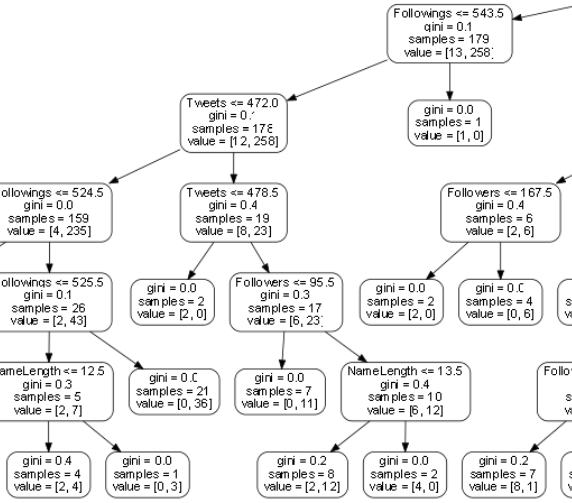
\includegraphics[width=100mm]{figures/decisiontree}
\caption{A section of a decision tree}
\end{figure}

\newpage
\section{Neural Network(NN) model}
The NN model works completely different compared to the random forest algorithms looked at until now. There are only two hyper-parameters, epochs and batch size. NN's tend to overfit after many epochs so it was important to find this point. The strategy was to first run the model for a large amount of epochs and see where the overfitting begins to happen, then only train the model for that specific length to get the best possible prediction.

\newpage

Here are the results of the accuracy and loss for both training and validation sets over 1000 epochs:
\begin{figure}[!h]
    \centering
	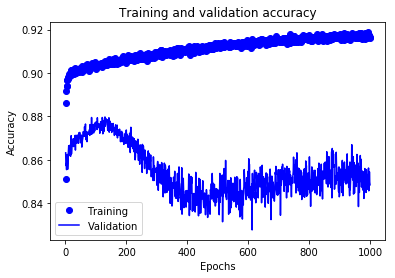
\includegraphics[width=100mm]{figures/accgraph}
	\caption{Accuracy over 1000 epochs}
\end{figure}
\begin{figure}[!h]
    \centering
	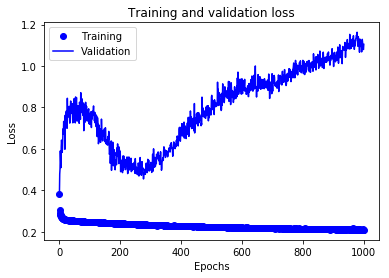
\includegraphics[width=100mm]{figures/lossgraph}
	\caption{Loss over 1000 epochs}
\end{figure}

In \textit{figure 6.1} the accuracy can be seen over the many epochs. The main focus is on the validation plots as that's the part that tells us how good the model is doing predicting new data. Initially the accuracy increases and around 150 epochs it cuts off and starts to decrease. That is roughly the point where overfitting starts to occur. We can confirm this by looking at the loss graph.

When it comes to the other graph, \textit{figure 6.2} we see the loss function, which we are trying to minimise to get rid of the errors. This figure is almost an inverted version of the accuracy one. The validation loss initially shoots up and then begins to decrease as the model is improving itself and adjusting to the data. At around 250 epochs in the validation loss begins to increase indefinitely. This is another major sign of overfitting and is telling us to stop. 

Using these two graphs we need to find a decent stopping point for when we retrain the model with a limited number of epochs then predict the labels of the test data that we put aside from the beginning. 

\begin{figure}[!h]
\centering
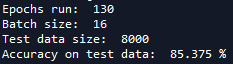
\includegraphics[width=100mm]{figures/nntestpredict}
\caption{Accuracy on test data after 130 epochs}
\end{figure}

\textit{Figure 6.3} shows the result of retraining the model for 130 epochs, then predicting the classes for the test data and comparing it to the actual labels given, which gives us 85.4\% accuracy. This is close to sklearn implementation but quite far off the other one, almost 10\% difference. Overall it's not a bad model as it outperforms randomly assigning the data labels which would result in a basic 50\% accuracy. The good thing about NN is it trains relatively fast and with a lot of data. This means potential future updates would be easy to complete compared to the random forest systems which took much longer. 



